%%%%%%%%%%%%%%%%%%%%%%%%%%%%%%%%%%%%%%%%%%%%%%%%%%%%%%%
% A template for Wiley article submissions.
% Developed by Overleaf. 
%
% Please note that whilst this template provides a 
% preview of the typeset manuscript for submission, it 
% will not necessarily be the final publication layout.
%
% Usage notes:
% The "blind" option will make anonymous all author, affiliation, correspondence and funding information.
% Use "num-refs" option for numerical citation and references style.
% Use "alpha-refs" option for author-year citation and references style.

\documentclass[alpha-refs]{wiley-article-05g}
% \documentclass[blind,num-refs]{wiley-article}

% Add additional packages here if required
\usepackage{siunitx}

% For figures
\usepackage{graphics}

%For captions - even though template has complex caption commands
\usepackage[labelfont=bf,justification=centering]{caption}
\usepackage[font=small,labelfont=bf]{subcaption}
\captionsetup[sub]{font=tiny,labelfont={bf,sf}}

%% For figures numbered by section
\usepackage{chngcntr}
\counterwithin{figure}{section}
\counterwithin{table}{section}

%% Additional links for hyperref
\usepackage[unicode=true,pdfusetitle,
 bookmarks=false,bookmarksnumbered=false,bookmarksopen=true,bookmarksopenlevel=2,
 breaklinks=false,pdfborder={0 0 1},backref=false,colorlinks=false]
 {hyperref}
\hypersetup{pdfstartview={XYZ null null 1}}

\usepackage[backend=bibtex,
			natbib=true, 
			style=chicago-authordate]{biblatex}
\addbibresource{Returns.bib}

\usepackage{array}
\usepackage{longtable}
%\usepackage{fullpage}

\usepackage{lmodern}
\newcommand{\graph}[3]{
\raisebox{-#1mm}{\includegraphics[height=#2em,width=3cm]{#3}}
}

\usepackage{booktabs} % for vertically partitioned table

\usepackage{lipsum}  % for fillers

%%%%%%%%#################################################################################%%%%%%%%%%%%%%%%%%%%%%%%%%%%%

% Update article type if known
\papertype{WORLD BANK EDUCATION GLOBAL PRACTICE}
% Include section in journal if known, otherwise delete
\paperfield{Russian Federation: Analytical Services and Advisory Activity: 
P170978}

\title{Returns to Education in the Russian Federation: Towards Evidence Based Decision Making with Social and Private Returns to Education}

% List acknowledgements here.
\fundinginfo{Thanks are due to the Ministry of Education and the Ministry of Finance for making the data available regarding graduate earnings and college and university income and expenditures. The code used for this paper is made freely available for all researchers at \url{https://bitbucket.org/zagamog/edreru/src/master/}}

% Include full author names and degrees, when required by the journal.
% Use the \authfn to add symbols for additional footnotes and present addresses, if any. Usually start with 1 for notes about author contributions; then continuing with 2 etc if any author has a different present address.

\author[*]{Ekaterina Melianova}
\author[*]{\hspace{-1em}Suhas Parandekar}
\author[*]{\hspace{-1em}Art\"{e}m Volgin}

% List abbreviations here, if any. Please note that it is preferred that abbreviations be defined at the first instance they appear in the text, rather than creating an abbreviations list.
\acks{\begin{normalsize}
\emph{Country Director:} Renaud Seligman; \emph{Regional Director:} Fadia Saadah; \emph{Practice Manager:} Harry Patrinos; \emph{Program Leader:} Dorota Nowak; \emph{Peer Reviewers}: Cristian Aedo; Ruslan Yemtsov; Husein Abdul-Hamid; \emph{Team members:} Polina Zavalina; Zhanna Terlyga. Thanks to seminar participants at the World Bank Moscow office on Jan. 29, 2020 for useful feedback. Any errors are a responsibility of the authors.
\end{normalsize}
\vspace{-0.2in}}

%\contrib[\authfn{1}]{Equally contributing authors.}

% Include full affiliation details for all authors
\affil[*]{Education Global Practice, Europe and Central Asia}

%\corraddress{Author One PhD, Department, Institution, City, State or Province, Postal Code, Country}
\corremail{sparandekar@worldbank.org}

%\presentadd[\authfn{2}]{Department, Institution, City, State or Province, Postal Code, Country}

% Include the name of the author that should appear in the running header
\runningauthor{P170978: WP05 - Private and Social Returns to Education}

\begin{document}

\maketitle

\begin{abstract}
This paper presents a preliminary analysis of a dataset distributed by the Ministry of Education of the Russian Federation that provides information on graduate salaries. The data is merged with information on income and fee revenue of colleges and universities to provide estimates of costs and benefits at an institutional level and private and social returns to education at a regional level. As the length of the data series on graduate earnings will grow over time, the estimates presented in this paper can be updated to provide sharper estimates of the costs and benefits of attending a particular institution.

% Please include a maximum of seven keywords
\keywords{Returns to Education, Higher Education, Cost-Benefit Analysis \emph{JEL Codes: I23, I26}}
\end{abstract}

\section{Description of Data}

The Ministry of Education provides information regarding  the salaries obtained by graduates and other related information at the website \hyperref[graduate.edu]{''http://graduate.edu.ru''}. A key purpose of this website is to provide accurate information to prospective university students and their families about the prospects of graduates from each of the universities or colleges. The Ministry of Finance collects information from all education establishments and others providing public service as a means to foster citizen engagement and accountability.This information includes details about revenue and income streams. This paper presents analysis from the merger of these two databases. The content of the data is presented in this section. Subsequent sections provide analysis and interpretation.

\subsection{Graduate.edu portal}

\textbf{One or two paragraphs explaining the process of data collection for graduate.edu}

\lipsum[1]

\textbf{Another sentence telling size of data - how many univs, colleges etc.} 

TABLE HERE OF DESCRIPTIVE STATISTICS OF THE VARIABLES

Column: Mean, Standard deviation and three quartiles - 25\% 50\% (or median) and 75\% and N 
6 Rows - College Natl.Average Graduate Earnings 2014; Earnings 2015;Earnings 2016;  Univ for 3 years



AV: Please color the two parts of the boxplots and introduce 3 or 4 vertical reference lines in the graph for easier reading; use the same scale please.



\begin{figure}[htbp!]
	\centering
	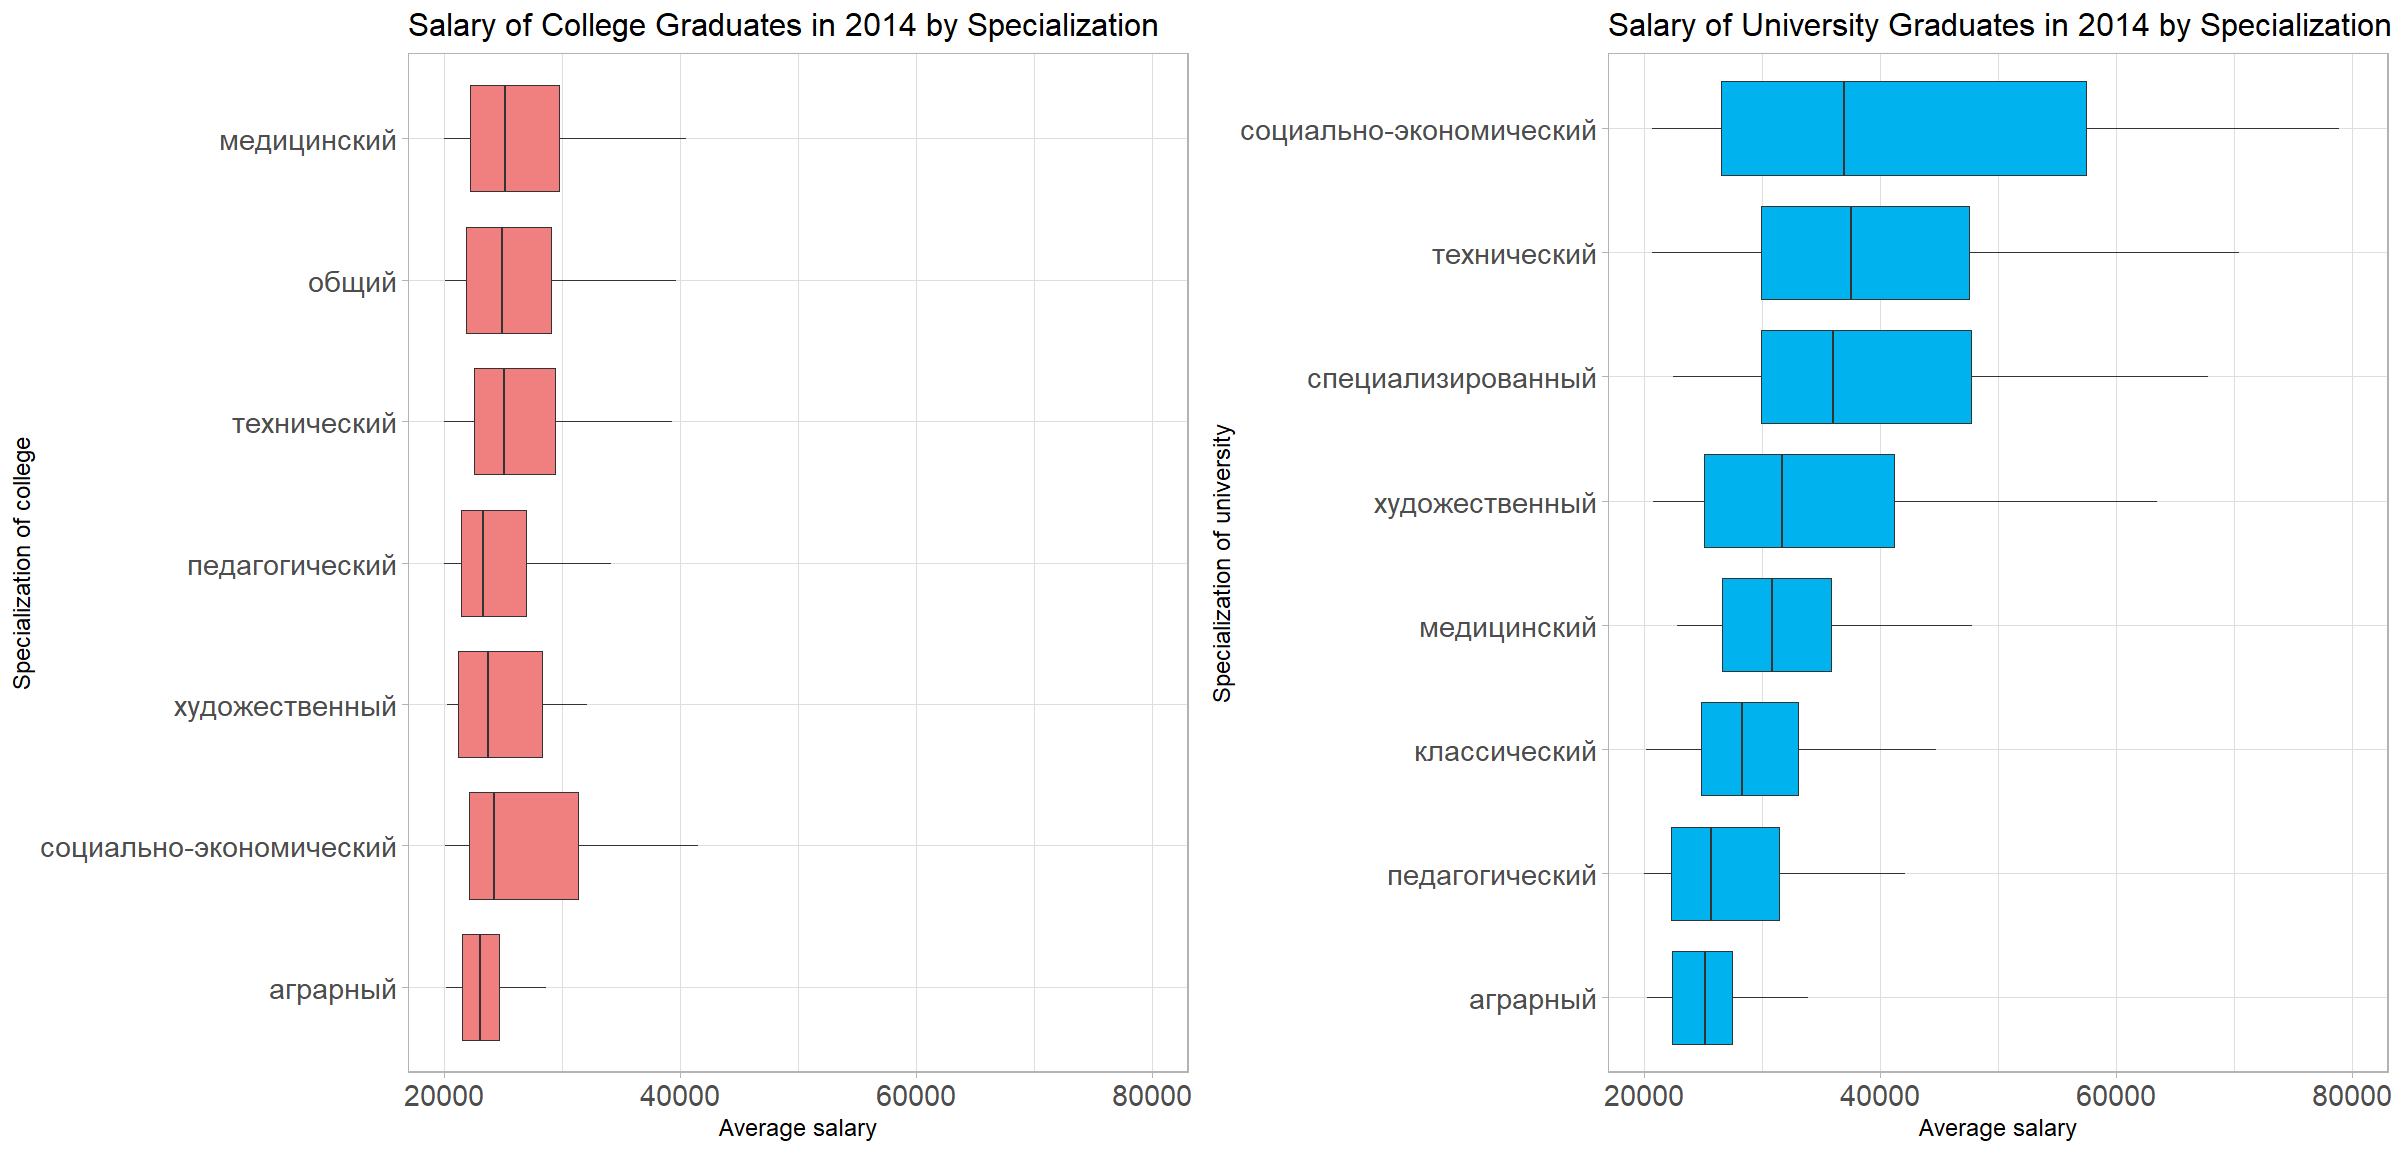
\includegraphics[width=400pt]{box_plot1a.png}
	\caption{Earnings in 2014 by Specialization}\label{fig:1.1}
\end{figure}



\textbf{Couple of sentence about growth in earnings in real terms over the period to introduce next figure}

Please change with line to connect the two dots and arrange in order of descending gap as we discussed on the Skype call. 




\begin{figure}[htbp!]
	\centering
	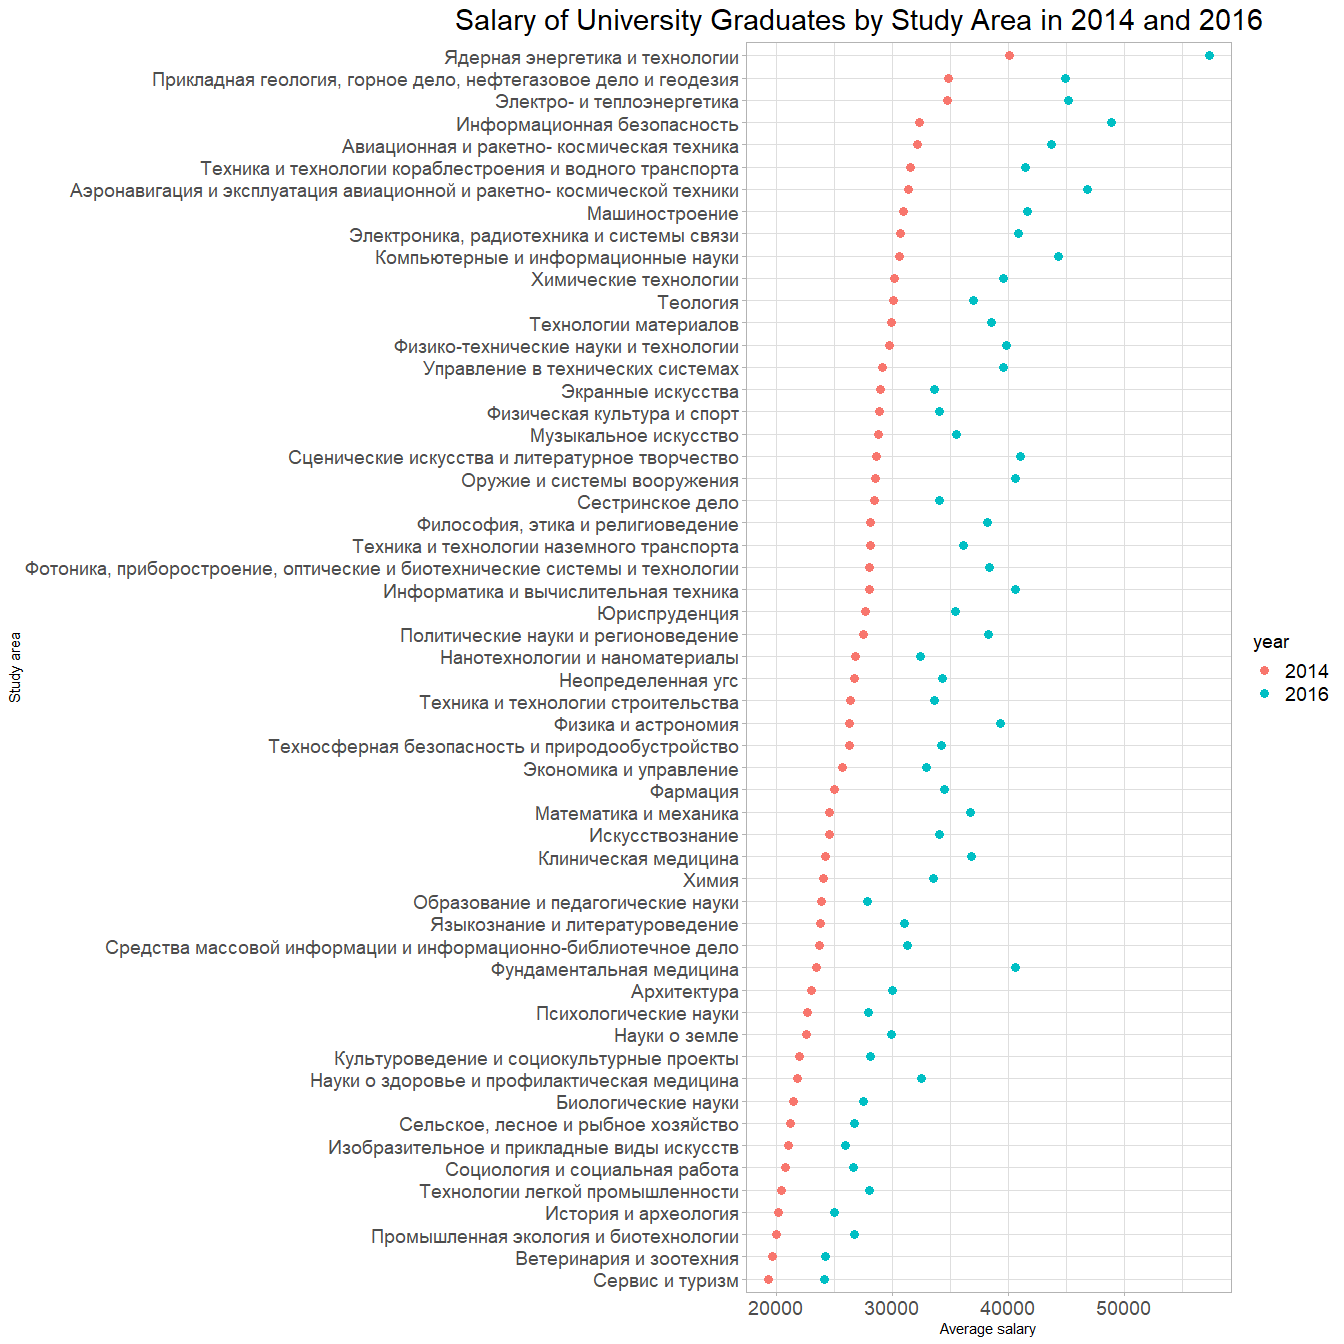
\includegraphics[width=400pt]{sal_inc.png}
	\caption{Earnings Growth 2014-16 by Specialization}\label{fig:1.2}
\end{figure}



\subsection{Bus.gov portal}

\lipsum[1] 

\textbf{Paragraph about contents of our bus.gov portal database}

TABLE Columns as before, Mean SD, 3 quartiles and Number of est
Rows - 8 each for college and 8 for university: 8 = 5 + 1 +2
5 cash receipt concepts including total (average across 6 years - if possible
use constant 2016 rubles but we can use nominal for now); 
1 row number of graduate
2 rows our unit cost figures private and social




\section{Institutional Returns for Colleges and Universities}

Explain the method we are using with a couple of equations. We will cite \cite{Psacharopoulos_1995}.

How many years to break even

Top/Bottom 10 as you have before also with column of break-even years

\begin{figure}[htbp!]
	\centering
	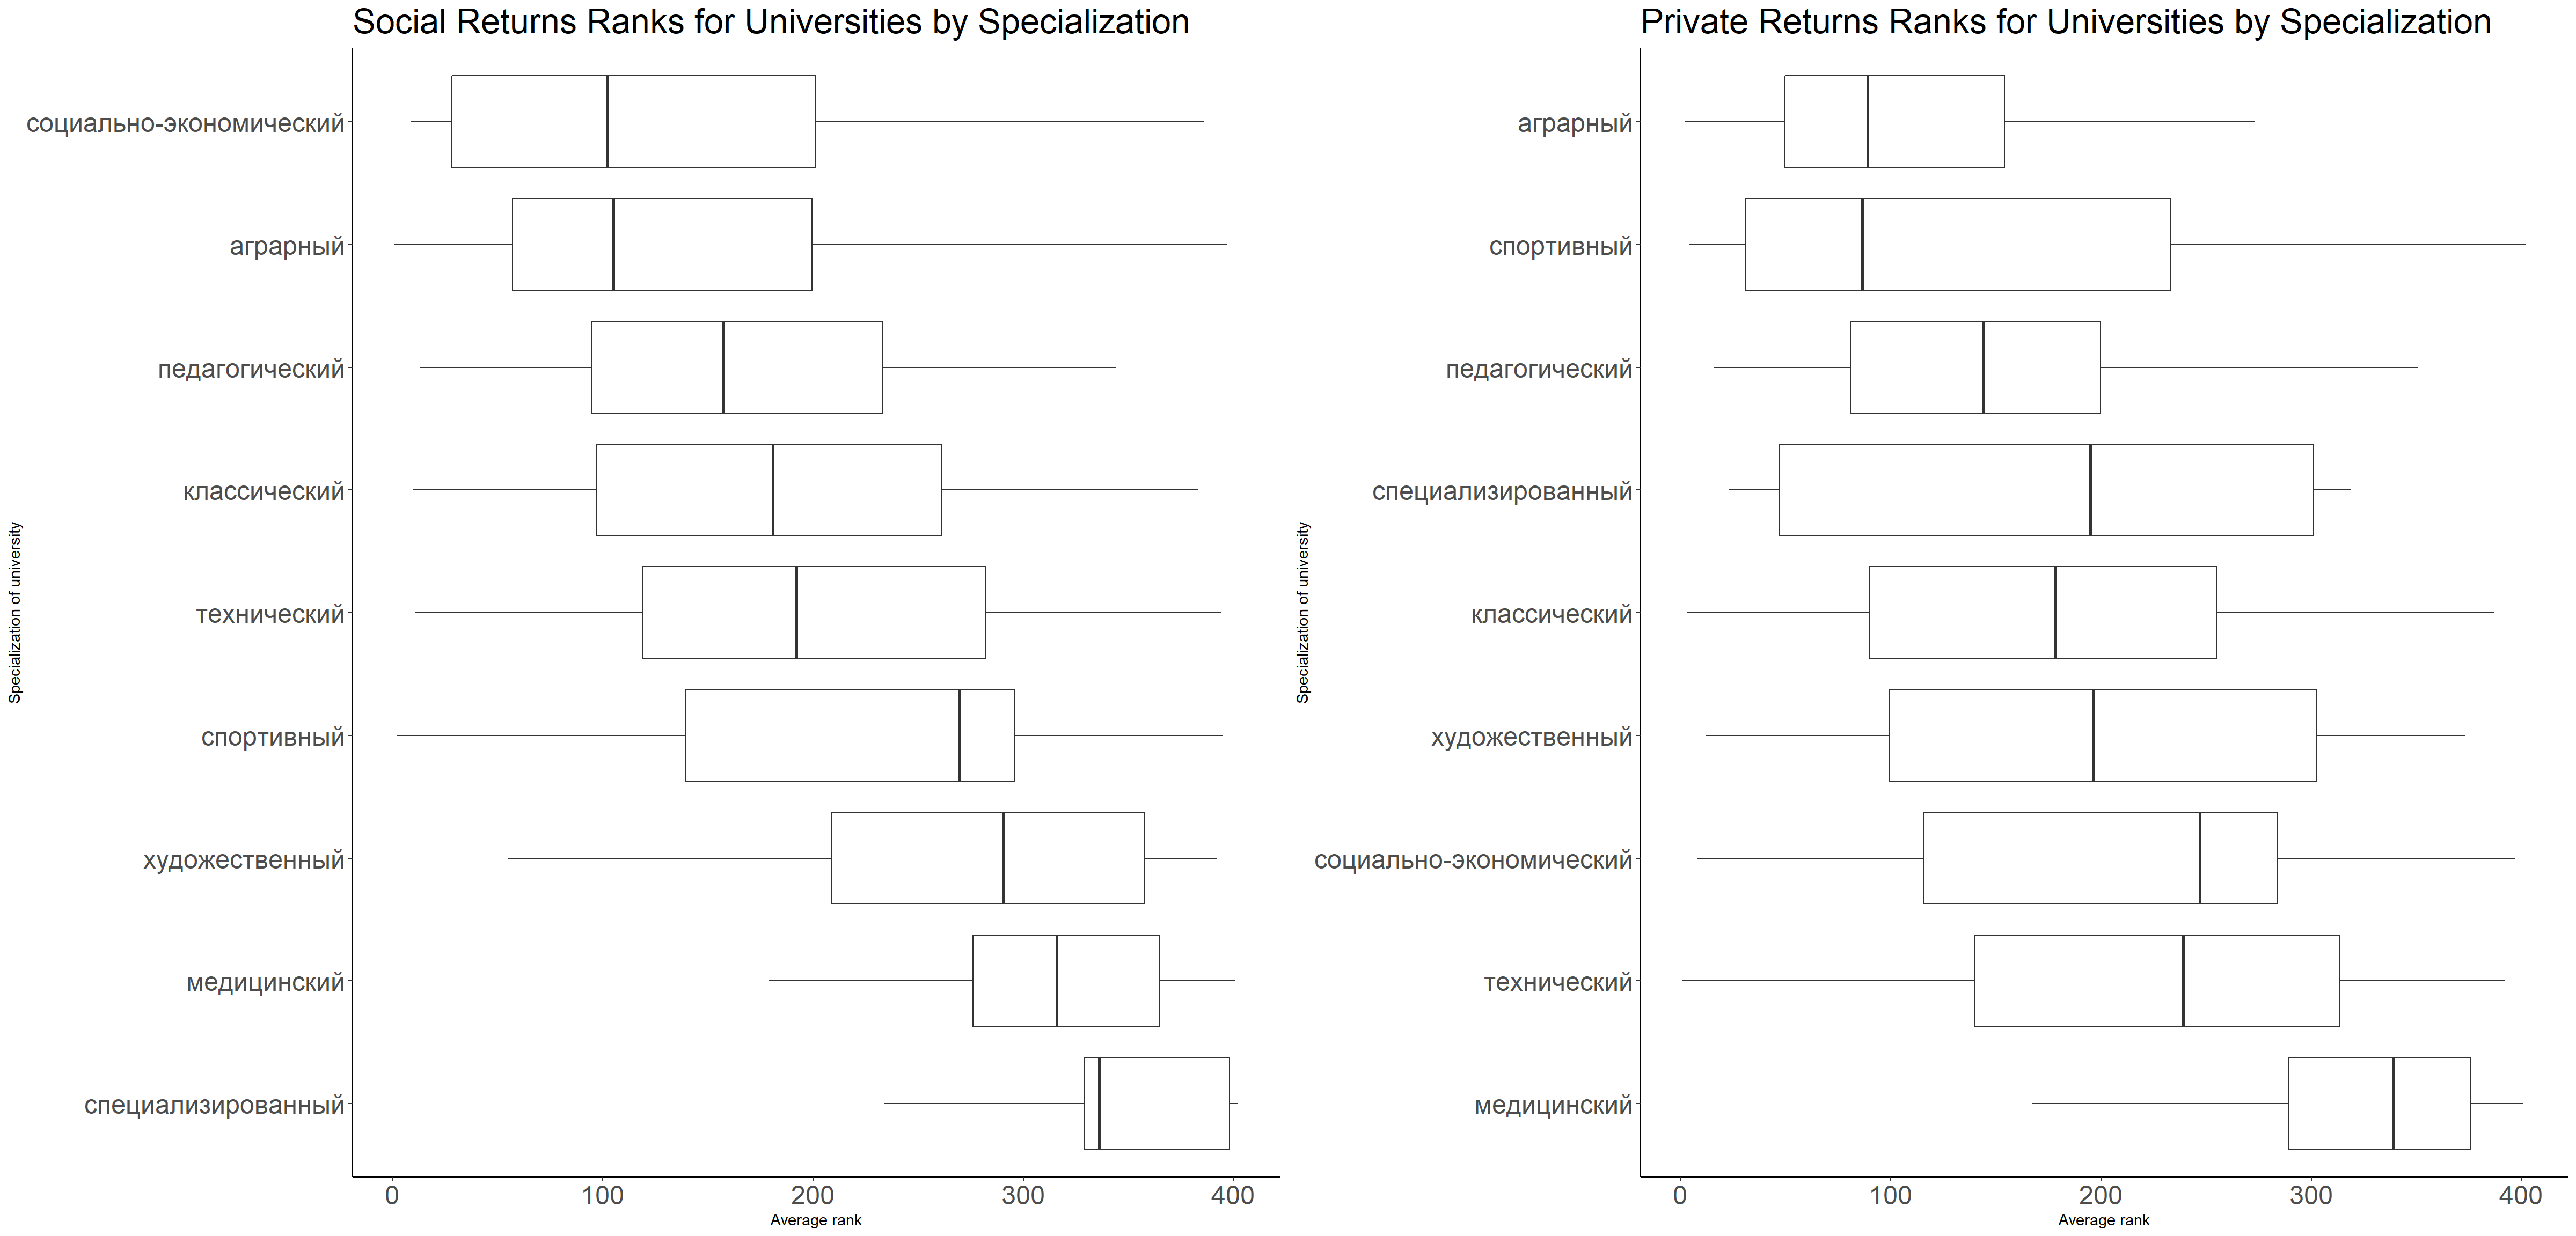
\includegraphics[width=400pt]{socret_uni.png}
	\caption{Soc Return Uni}\label{fig:2.1}
\end{figure}


\begin{figure}[htbp!]
	\centering
	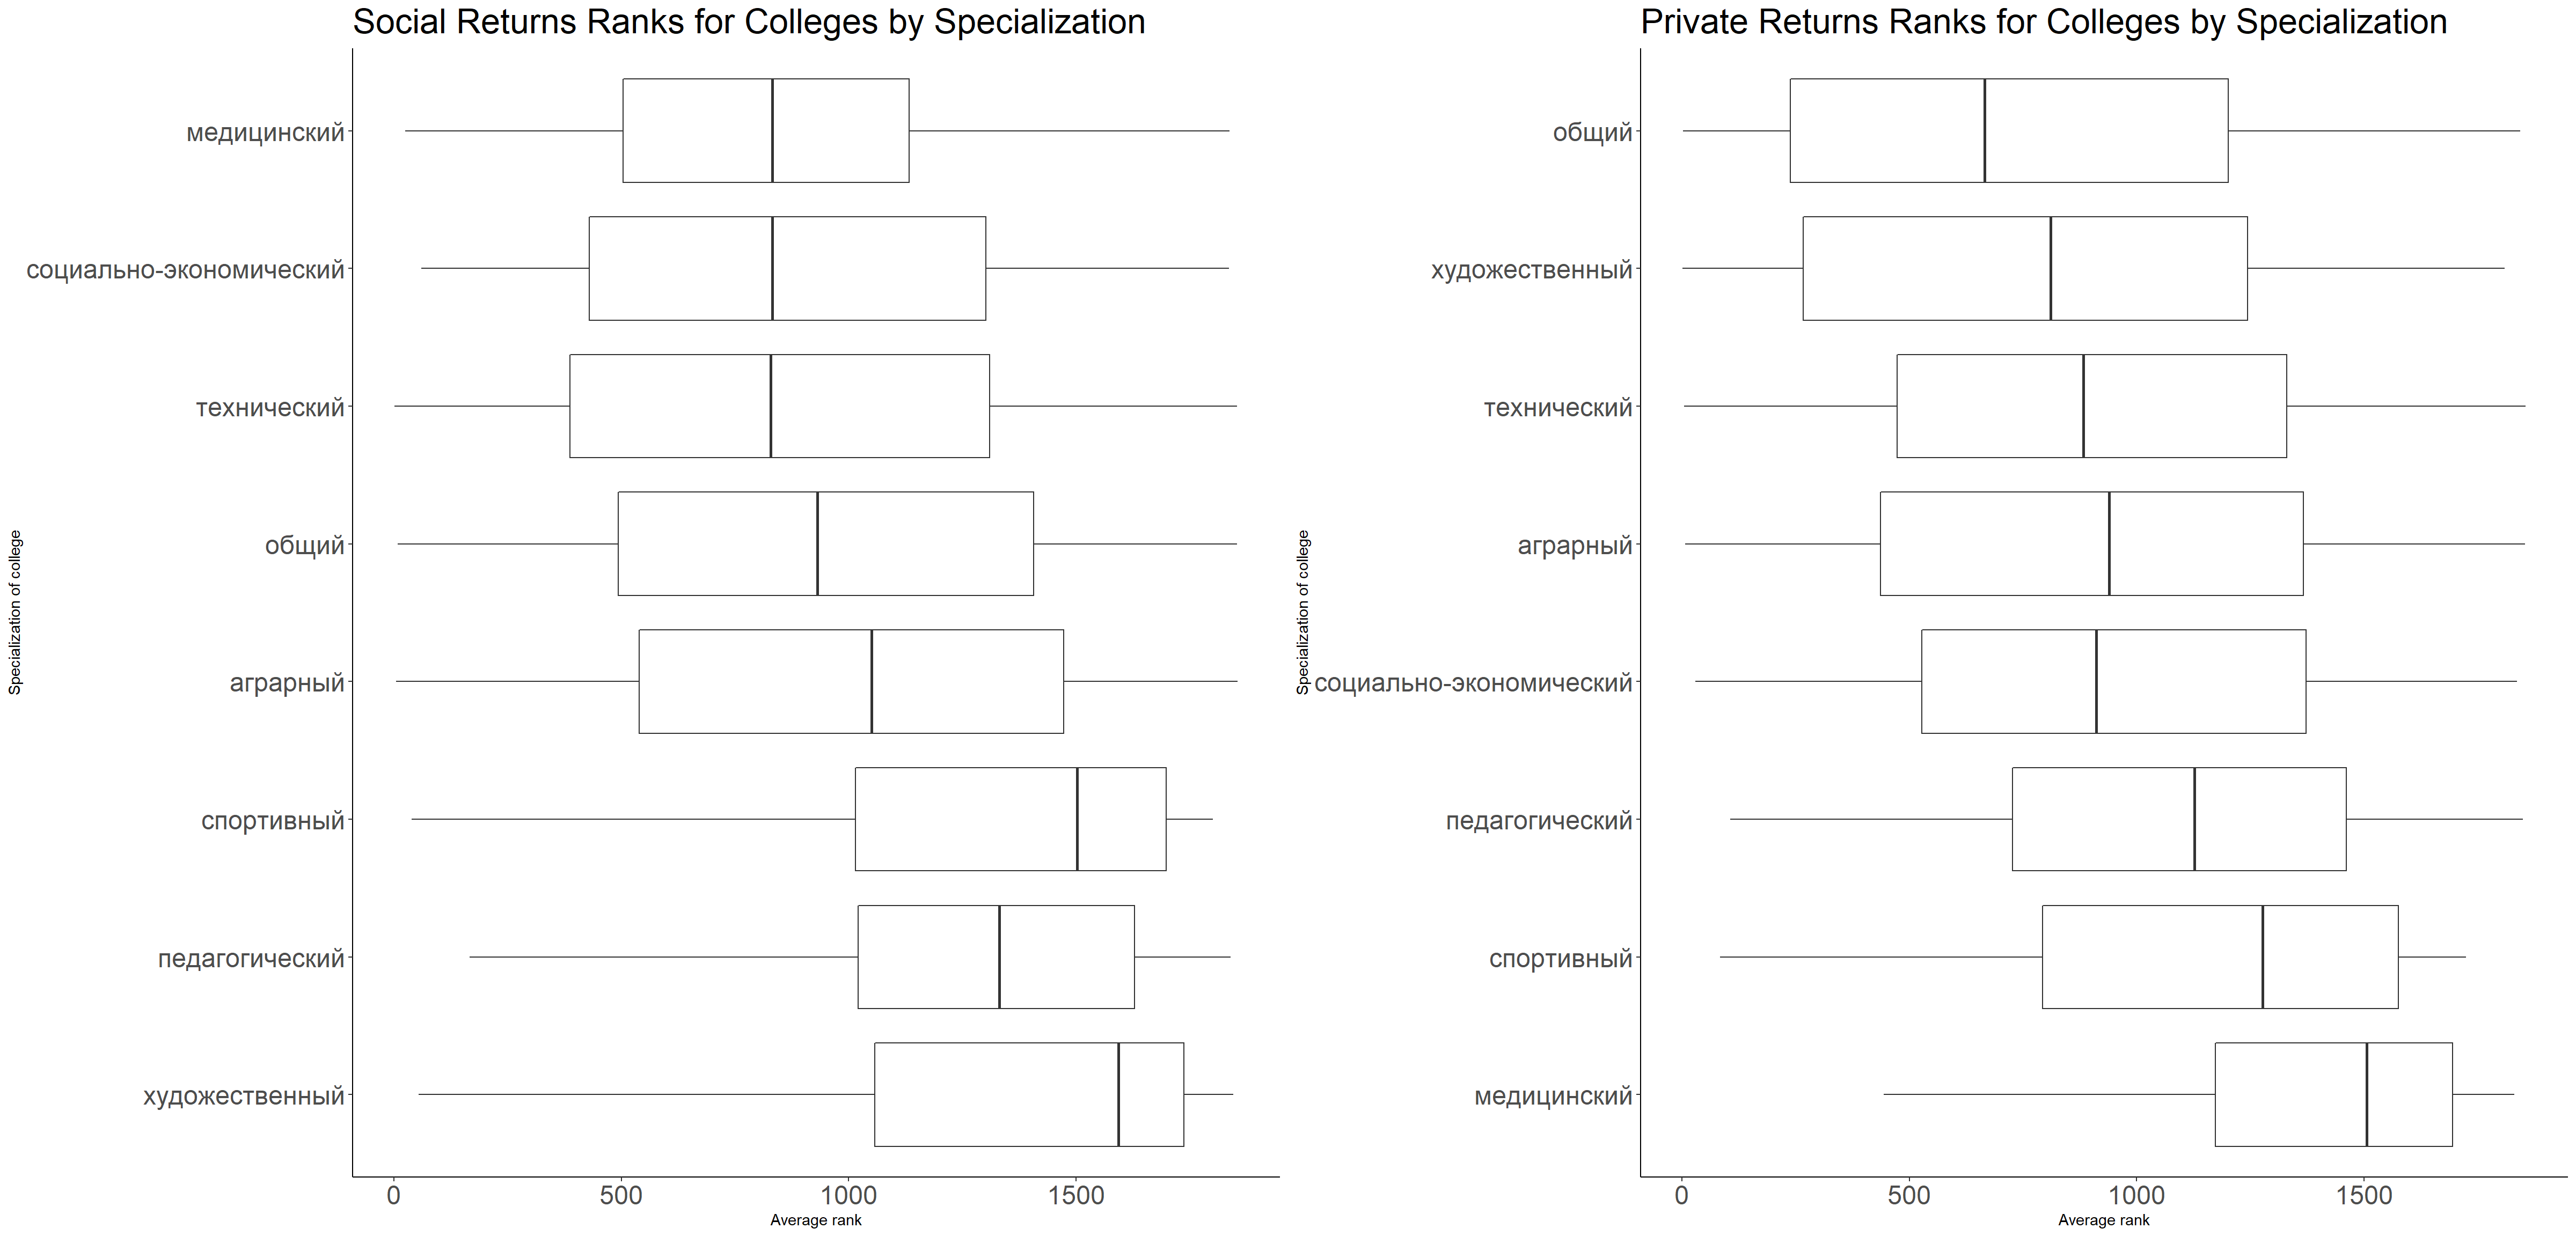
\includegraphics[width=400pt]{socret_col.png}
	\caption{Priv Return Uni}\label{fig:2.2}
\end{figure}

And same for college

\lipsum[2]

\lipsum[3]

\section{Regional Estimates of Social and Private Returns}

\lipsum[4]

Here we calculate age earnings profiles at regional level from Rosstat = Let's use 2013 to 2018 average in real 2018 rubles for each age to calculate the profile.

Then we total the cost figures at institution level for that region to get our first 3 or 4 negative numbers for average private and social cost of education 
Then full method gives us returns. We could provide simulated errors but I don't see much point, we will just present the points in a snake diagram or whatever you call it regions arranged by descending returns; one for college and one for universities.

If time allows, we will add about migration and something about quality from EGE score data.

\printbibliography

\newpage
\section*{Appendix}
\addcontentsline{toc}{section}{Appendix}%

\setcounter{table}{0}
\renewcommand{\thetable}{A\arabic{table}}


\begin{table}[!htbp] \centering 
\caption{Results of Estimating Human Capital Depreciation for the Female sample, RLMS} 
	\label{tab:A1}
\begin{tabular}{@{\extracolsep{5pt}}lcccccc} 
\\[-1.8ex]\hline 
\hline \\[-1.8ex] 
& \textbf{1994} & \textbf{1998} & \textbf{2003} & \textbf{2006} & \textbf{2012} & \textbf{2018} \\ 
\\[-1.8ex] & (1) & (2) & (3) & (4) & (5) & (6)\\ 
\hline \\[-1.8ex] 
 Constant & 9.725$^{***}$ & 3.786$^{***}$ & 5.464$^{***}$ & 6.946$^{***}$ & 8.133$^{***}$ & 8.767$^{***}$ \\ 
  & (0.381) & (0.322) & (0.301) & (0.247) & (0.186) & (0.242) \\ 
  & & & & & & \\ 
 Educ, years ($S$) & 0.122$^{***}$ & 0.153$^{***}$ & 0.158$^{***}$ & 0.118$^{***}$ & 0.087$^{***}$ & 0.066$^{***}$ \\ 
  & (0.025) & (0.022) & (0.020) & (0.016) & (0.012) & (0.015) \\ 
  & & & & & & \\ 
 Educ X Exper ($TS$) & $-$0.002$^{*}$ & $-$0.002$^{***}$ & $-$0.002$^{**}$ & $-$0.0002 & $-$0.0001 & 0.0004 \\ 
  & (0.001) & (0.001) & (0.001) & (0.001) & (0.0005) & (0.001) \\ 
  & & & & & & \\ 
 Exper ($T$) & 0.074$^{***}$ & 0.080$^{***}$ & 0.055$^{***}$ & 0.013 & 0.020$^{**}$ & 0.020$^{*}$ \\ 
  & (0.019) & (0.016) & (0.015) & (0.013) & (0.010) & (0.011) \\ 
  & & & & & & \\ 
 Exper squared ($T^2$) & $-$0.001$^{***}$ & $-$0.001$^{***}$ & $-$0.001$^{***}$ & $-$0.0003$^{**}$ & $-$0.0005$^{***}$ & $-$0.001$^{***}$ \\ 
  & (0.0002) & (0.0002) & (0.0002) & (0.0001) & (0.0001) & (0.0001) \\ 
  & & & & & & \\ 
\hline \\[-1.8ex] 
Observations & 1,645 & 1,667 & 2,093 & 2,630 & 4,057 & 3,312 \\ 
R$^{2}$ & 0.051 & 0.089 & 0.110 & 0.139 & 0.104 & 0.092 \\ 
Adjusted R$^{2}$ & 0.049 & 0.087 & 0.108 & 0.138 & 0.103 & 0.091 \\ 
Residual Std. Error & 0.853 & 0.728 & 0.731 & 0.664 & 0.641 & 0.597 \\ 
F Statistic & 22.179$^{***}$ & 40.520$^{***}$ & 64.342$^{***}$ & 106.385$^{***}$ & 117.366$^{***}$ & 83.993$^{***}$ \\ 
\hline 
\hline \\[-1.8ex] 
\textit{Note:}  & \multicolumn{6}{r}{$^{*}$p$<$0.1; $^{**}$p$<$0.05; $^{***}$p$<$0.01} \\ 
\end{tabular} 
\end{table} 


\begin{table}[!htbp] \centering 
\caption{Results of Estimating Human Capital Depreciation for the Male sample, RLMS} 
	\label{tab:A2}
\begin{tabular}{@{\extracolsep{5pt}}lcccccc} 
\\[-1.8ex]\hline 
\hline \\[-1.8ex] 
& \textbf{1994} & \textbf{1998} & \textbf{2003} & \textbf{2006} & \textbf{2012} & \textbf{2018} \\ 
\\[-1.8ex] & (1) & (2) & (3) & (4) & (5) & (6)\\ 
\hline \\[-1.8ex] 
 Constant & 10.357$^{***}$ & 5.029$^{***}$ & 7.334$^{***}$ & 8.067$^{***}$ & 8.771$^{***}$ & 9.094$^{***}$ \\ 
  & (0.433) & (0.360) & (0.282) & (0.243) & (0.157) & (0.185) \\ 
  & & & & & & \\ 
 Educ, years ($S$) & 0.136$^{***}$ & 0.123$^{***}$ & 0.080$^{***}$ & 0.077$^{***}$ & 0.077$^{***}$ & 0.077$^{***}$ \\ 
  & (0.028) & (0.024) & (0.019) & (0.016) & (0.010) & (0.012) \\ 
  & & & & & & \\ 
 Educ X Exper ($TS$) & $-$0.002$^{*}$ & $-$0.001 & 0.0004 & $-$0.0003 & $-$0.0004 & $-$0.001 \\ 
  & (0.001) & (0.001) & (0.001) & (0.001) & (0.0005) & (0.001) \\ 
  & & & & & & \\ 
 Exper ($T$) & 0.054$^{**}$ & 0.032$^{*}$ & 0.002 & 0.007 & 0.035$^{***}$ & 0.037$^{***}$ \\ 
  & (0.023) & (0.017) & (0.014) & (0.013) & (0.009) & (0.010) \\ 
  & & & & & & \\ 
 Exper squared ($T^2$) & $-$0.001$^{***}$ & $-$0.0004$^{**}$ & $-$0.0003$^{*}$ & $-$0.0003$^{*}$ & $-$0.001$^{***}$ & $-$0.001$^{***}$ \\ 
  & (0.0003) & (0.0002) & (0.0002) & (0.0001) & (0.0001) & (0.0001) \\ 
  & & & & & & \\ 
\hline \\[-1.8ex] 
Observations & 1,392 & 1,433 & 1,763 & 2,170 & 3,360 & 2,800 \\ 
R$^{2}$ & 0.057 & 0.070 & 0.078 & 0.074 & 0.153 & 0.110 \\ 
Adjusted R$^{2}$ & 0.054 & 0.067 & 0.076 & 0.072 & 0.152 & 0.108 \\ 
Residual Std. Error & 0.951 & 0.803 & 0.754 & 0.688 & 0.598 & 0.570 \\ 
F Statistic & 20.989$^{***}$ & 26.879$^{***}$ & 37.362$^{***}$ & 43.281$^{***}$ & 151.868$^{***}$ & 86.125$^{***}$ \\ 
\hline 
\hline \\[-1.8ex] 
\textit{Note:}  & \multicolumn{6}{r}{$^{*}$p$<$0.1; $^{**}$p$<$0.05; $^{***}$p$<$0.01} \\ 
\end{tabular} 
\end{table} 



\newpage
\printbibliography

\end{document}
